\documentclass[10pt]{article}

% Packages
\usepackage[a4paper,
            left=0.5in,
            right=0.5in,
            top=0.5in,
            bottom=1in]{geometry}\usepackage{graphicx}

\setlength\parindent{0pt}

\usepackage{enumitem}
\usepackage{textcomp}
\usepackage{gensymb}
\usepackage{amsmath}
\usepackage{amssymb}
\usepackage{amsfonts}

\usepackage{esint}
\usepackage{tikz}
\usepackage{pgfplots}
\pgfplotsset{compat=newest}
\usepackage{pgfplotstable}

\usepackage{subcaption}
\usepackage{graphicx}

\usepackage{setspace} 

\usepackage{physics}

\DeclareCaptionLabelSeparator{titik}{. }

\begin{document}
\captionsetup[figure]{labelfont={sc}, labelsep=titik}

\begin{center}
    \textbf{AE2202 Fluid Dynamics} \\
    \textbf{Homework 6}
\end{center}

\hfill

\textbf{Question 1}. A solid circular cylinder of radius $R$ rotates at angular velocity $\Omega$ in a viscous incompressible fluid that is at rest far from the cylinder, as in figure below. Make simplifying assumptions and derive the governing differential equation and boundary conditions for the velocity field $v_\theta$ in the fluid. What is the steady-state flow field for this problem?

\begin{figure}[h]
    \centering
    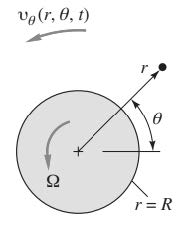
\includegraphics{Problem1.jpg}
    \caption{Illustration of Problem 1}
    \label{fig:figprob1}
\end{figure}

\textbf{\underline{Answer}}

Based on the description, the fluid surrounding the cylinder is viscous and incompressible and we only consider steady-sate condition. To simplify even further, we will assume (1) the fluid only move in the direction of $\theta$ and (2) uniform pressure distribution. We also have our boundary condition to be (1) the relative velocity of the fluid at the surface of the cylinder with respect the surfce is zero and (2) the velocity of the fluid far from the surface is zero. We have our governing equation of Navier-Stokes Theorem:
\begin{equation}
    \rho \frac{d \mathbf{v}}{dt} = -\mathbf{\nabla}p + \mu \nabla^2 \mathbf{v} + \rho \mathbf{g}
\end{equation}
For cylindrical coordinates at $\theta$,
\begin{equation}
    \rho\left( \frac{\partial v_\theta}{\partial t} + v_r \frac{\partial v_\theta}{\partial r} + \frac{1}{r} v_\theta \frac{\partial v_\theta}{\partial \theta} + v_z \frac{\partial v_\theta}{\partial z} + \frac{v_r v_\theta}{r}\right) = -\frac{1}{r} \frac{\partial p}{\partial \theta} + \mu \left(\frac{1}{r} \frac{\partial}{\partial r}\left(r \frac{\partial v_\theta}{\partial r}\right) + \frac{1}{r^2} \frac{\partial^2 v_\theta}{\partial \theta^2} + \frac{\partial^2 v_\theta}{\partial z^2} + \frac{2}{r^2} \frac{\partial v_\theta}{\partial \theta} - \frac{v_\theta}{r^2}\right) + \rho g_\theta
\end{equation}
Applying our assumptions,
\begin{align*}
    0 + 0 + 0 + 0 + 0 &= 0 + \mu \left(\frac{1}{r} \frac{\partial}{\partial r}\left(r \frac{\partial v_\theta}{\partial r}\right) + 0 + 0 + 0 - \frac{v_\theta}{r^2}\right) + 0 \\
    \frac{1}{r} \frac{\partial}{\partial r}\left(r \frac{\partial v_\theta}{\partial r}\right) - \frac{v_\theta}{r^2} &= 0 \\
    \frac{\partial^2 v_\theta}{\partial r^2} + \frac{1}{r} \frac{\partial v_\theta}{\partial r} - \frac{v_\theta}{r^2} &= 0 \\
    r^2 \frac{\partial^2 v_\theta}{\partial r^2} + r \frac{\partial v_\theta}{\partial r} - v_\theta &= 0\hspace{8pt}\left[\textrm{Euler-Cauchy Equation}\right] \\
    v_\theta (r) &= c_1 r + \frac{c_2}{r} 
\end{align*}
Rewriting our boundary conditions:
\begin{enumerate}
    \item $(v_\theta (R))_{\textrm{rel}} = 0 \Rightarrow v_\theta (R) = \Omega R$
    \item $\lim_{r \rightarrow \infty} (v_\theta (r)) = 0$
\end{enumerate}
For that BC 2. is valid, $c_1$ must be zero to ensure $v_\theta (r)$ not diverging to invinity when $r \rightarrow 0$. Thus,
\begin{align*}
    \Omega R &= \frac{c_2}{R} \\
    c_2 &= \Omega R^2
\end{align*}
Therefore, we got that
\begin{equation*}
    v_\theta (r) = \frac{\Omega R^2}{r}
\end{equation*}

\break

\textbf{Question 2}. Two immiscible liquids of equal thickness $h$ are being sheared between a fixed and a moving plate, as in figure below. Gravity is neglected and there is no variation with $x$. Find an expression for:
\begin{enumerate}[label=\arabic*), noitemsep, nosep]
    \item the velocity at the interface.
    \item the shear stress in each fluid.
\end{enumerate}
Assume steady laminar flow.

\begin{figure}[h]
    \centering
    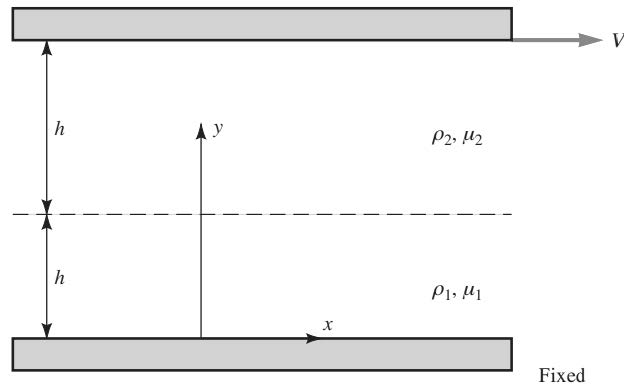
\includegraphics[scale=0.83]{Problem2.jpg}
    \caption{Illustration of Problem 2}
    \label{fig:figprob2}
\end{figure}

\textbf{\underline{Answer}}

Assumptions:
\begin{enumerate}[noitemsep, nosep]
    \item Steady state
    \item Laminar flow
    \item Incompressible liquid
    \item The fluids only move in the direction of $x$
    \item Gravity is negligible
    \item No variation of fluids in the $x$ direction
    \item Uniform pressure accross $x$
\end{enumerate}

\hfill

Governing Equation:
\begin{enumerate}[noitemsep, nosep]
    \item Navier-Stokes Theorem
    \begin{equation}
        \rho \frac{d \mathbf{v}}{dt} = -\mathbf{\nabla}p + \mu \nabla^2 \mathbf{v} + \rho \mathbf{g}
    \end{equation}

    and in Cartesian coordinate system, in $x-$direction
    \begin{equation}
        \rho \left( \frac{\partial v_x}{\partial t} + v_x \frac{\partial v_x}{\partial x} + v_y \frac{\partial v_x}{\partial y} + v_z \frac{\partial v_x}{\partial z} \right) = -\frac{\partial p}{\partial x} + \mu \left(\frac{\partial^2 v_x}{\partial x^2} + \frac{\partial^2 v_x}{\partial y^2} + \frac{\partial^2 v_x}{\partial z^2} \right) + \rho g_x
    \end{equation}
\end{enumerate}

\hfill

Analysis: \\
Using (4) with our assumptions, for one liquid:
\begin{align*}
    \rho(0 + 0 + 0 + 0) &= -0 + \mu(0 + \frac{\partial^2 v_x}{\partial y^2} + 0) + 0 \\
    \frac{\partial^2 v_x}{\partial y^2} &= 0 \\
    \frac{\partial v_x}{\partial y} &= c_1 \\
    v_x(y) &= c_1 y + c_2
\end{align*}

As we can see here, the distribution of fluid is linear, buth should have different slope for different fluid. Our boundary conditions are:
\begin{enumerate}
    \item At $y = 0$, liquid 1 doesn't move with respect to the lower surface $\rightarrow v_x(0) = 0$.
    \item At $y = h$ or at the interface, both liquid should move at the same rate (interface velocity, $v_x(h) = v_i$), and occurs a certain value of shear stress $\tau_1 (y = h) = \tau_2(y = h)$.
    \item At $y = 2h$, liquid 2 doesn't move with respect to the upper surface $\rightarrow v_x(2h) = V$.
\end{enumerate}

Therefore, we got that
\begin{align*}
    \tau_1 (y = h) &= \tau_2 (y = h) \\
    \mu_1 \frac{\partial (v_x)_1}{\partial y} &= \mu_2 \frac{\partial (v_x)_2}{\partial y} \\
    \mu_1 \frac{v_i - 0}{h - 0} &= \mu_2 \frac{V - v_i}{2h - h} \\
    \mu_1 v_i &= \mu_2 (V - v_i) \\
    v_i &= \frac{\mu_2}{\mu_1 + \mu_2} V
\end{align*}

From the derivation, we can see that the shear stress is actually a constant. Thus, the shear stress is same all over both liquid. We may find an expression of the shear stress with
\begin{align*}
    \tau_1 = \tau_2 := \tau = \tau_1 (y = h) &= \mu_1 \frac{\partial (v_x)_1}{\partial y} \\
    &= \mu_1 \frac{v_i}{h} \\
    &= \mu_1 \cdot \frac{\mu_2}{\mu_1 + \mu_2} \frac{V}{h} \\
    \tau &= \frac{\mu_1 \mu_2}{\mu_1 + \mu_2} \frac{V}{h}
\end{align*}

\break

\textbf{Question 3}. In the laminar flow a fluid in a circular pipe, the velocity profile is exactly a parabola. The rate of discharge is then represented by volume of a paraboloid. Prove that for this case the ratio of the maximum velocity to mean velocity is 2.

\hfill

\textbf{\underline{Answer}}

% ilustasi

The velocity profile of the fluid should be a circular paraboloid with a maximum value of maximum velocity ($V_{\textrm{max}}$) at the middle ($r = 0$) and have zero velocity on the inside surface of the pipe ($r = R$), and thus independent of the which direction from the center of the pipe (independent of $\theta$). We may represent the paraboloid function of the velocity with
\begin{equation}
    v_z(r) = V_{\textrm{max}} \left[1 - \left(\frac{r}{R}\right)^2\right]
\end{equation}
The volume of the paraboloid may be calculated with
\begin{align*}
    \textrm{V} &= \int_0^{2\pi} \int_0^R v_z(r)\ r\ dr\ d\theta \\
    &= 2\pi \int_0^R V_{\textrm{max}} \left[1 - \left(\frac{r}{R}\right)^2\right]r\ dr \\
    &= 2\pi V_{\textrm{max}} \int_0^R \left[r - \frac{r^3}{R^2}\right] dr \\
    &= 2\pi V_{\textrm{max}} \eval*{\frac{r^2}{2} - \frac{r^4}{4R^2}}_{0}^{R} \\
    &= 2\pi V_{\textrm{max}} \left(\frac{R^2}{4}\right) \\
    &= \frac{\pi R^2}{2} V_{\textrm{max}} \\
    &= \frac{A}{2} V_{\textrm{max}}
\end{align*}
The mean velovity is calculated so that the product of the mean velocity and the area of the pipe is the same as the volume calculated above.
\begin{align*}
    V_{\textrm{mean}} A &= \textrm{V} \\
    V_{\textrm{mean}} A &= \frac{A}{2} V_{\textrm{max}} \\
    \therefore \frac{V_{\textrm{max}}}{V_{\textrm{mean}}} &= 2
\end{align*}

\break

\textbf{Question 4}. A circular pipe of radius $a$ and length $L$ is attached to a smoothly rounded outlet of a liquid reservoir by means of flanges and bolts as shown in figure below. At the flange section the velocity is uniform over the cross-section with magnitude $V_0$. At the outlet, which discharges into the atmosphere, the velocity profile is parabolic because of the friction in the pipe. What force must be supplied by the bolts to hold the pipe in place?

\begin{figure}[h]
    \centering
    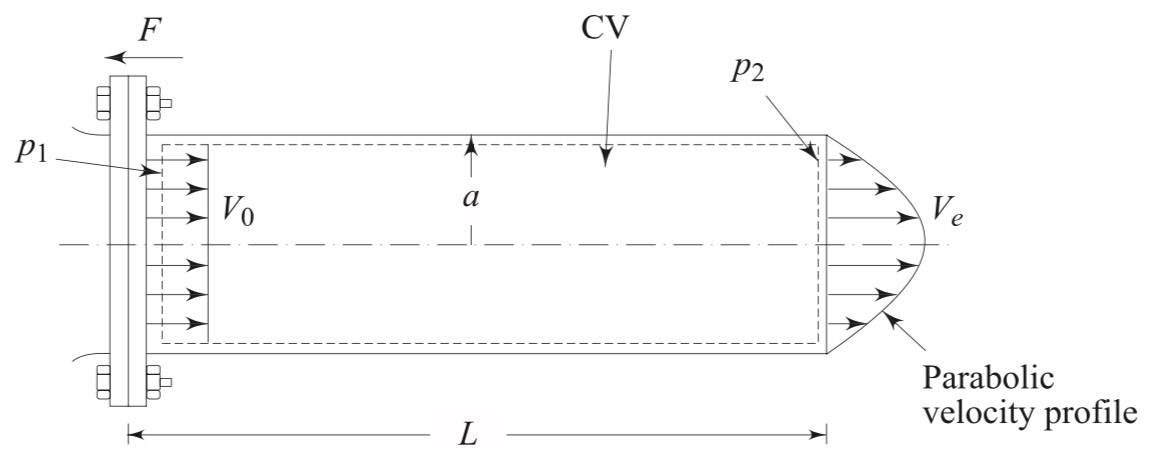
\includegraphics[scale=0.83]{Problem4.jpg}
    \caption{Illustration of Problem 4}
    \label{fig:figprob4}
\end{figure}

\textbf{\underline{Answer}}

Assumptions:
\begin{enumerate}[noitemsep, nosep]
    \item Incompressible fluid
    \item Steady state flow
\end{enumerate}

\hfill

Governing Equation:
\begin{enumerate}[noitemsep, nosep]
    \item Conservation of Mass
    \begin{equation}
        \frac{d m_{CV}}{dt} = -\oiint_{A_{CV}} \rho\left(\mathbf{v}_r \cdot \mathbf{\hat{n}}\right) dA
    \end{equation}

    \item Navier-Stokes Equation
    \begin{equation}
        \rho\left(\frac{\partial \mathbf{v}}{\partial t} + \left(\mathbf{v} \cdot \nabla\right) \mathbf{v}\right) = -\nabla p + \mu \nabla^2 \mathbf{v} + \rho\mathbf{g}
    \end{equation}

    For cylindrical coordinates at $z$,
    \begin{equation}
        \rho\left(\frac{\partial v_z}{\partial t} + v_r \frac{\partial v_z}{\partial r} + \frac{v_\theta}{r} \frac{\partial v_z}{\partial \theta} + v_z \frac{\partial v_z}{\partial z}\right) = -\frac{\partial p}{\partial z} + \mu \left(\frac{1}{r} \frac{\partial}{\partial r} \left(r \frac{\partial v_z}{\partial r}\right) + \frac{1}{r^2} \frac{\partial^2 v_z}{\partial \theta^2} + \frac{\partial^2 v_z}{\partial z^2}\right) + \rho g_z
    \end{equation}

    \item Conservation of Linear Momentum
    \begin{equation}
        \frac{d \mathbf{p}_{CV}}{dt} = F_{\textrm{body}} + F_{p} + F_{\textrm{viscous}} -\oiint_{A_{CV}} \rho \mathbf{v}\left(\mathbf{v}_r \cdot \mathbf{\hat{n}}\right) dA
    \end{equation}
\end{enumerate}

\hfill

Analysis:

Using (6), as the velocity profile is parabolic,
\begin{align*}
    0 &= -\iint_{A_{1}} \rho\left(\mathbf{v}_r \cdot \mathbf{\hat{n}}\right) dA +\iint_{A_{2}} \rho\left(\mathbf{v}_r \cdot \mathbf{\hat{n}}\right) dA \\
    \iint_{A_{1}} \left(\mathbf{v}_r \cdot \mathbf{\hat{n}}\right) dA &= \iint_{A_{2}} \left(\mathbf{v}_r \cdot \mathbf{\hat{n}}\right) dA \\
    V_0 \left(\pi a^2\right) &= \int_{0}^{a} V_e (r) \left(2\pi r\right) dr  \\
    \frac{1}{2} V_0 a^2 &= \int_{0}^{a} V_{\textrm{max}} \left[1 - \left(\frac{r}{a}\right)^2\right] r\ dr \\
    \frac{1}{2} V_0 a^2 &= \frac{V_{\textrm{max}}}{2} \left(\frac{a^2}{2}\right) \\
    V_{\textrm{max}} &= 2V_0
\end{align*}

Using (8) and our assumptions,
\begin{align*}
    \rho\left(0 + 0 + 0 + 0 + v_z \frac{\partial v_z}{\partial z}\right) &= -\frac{\partial p}{\partial z} + \mu \left(\frac{1}{r} \frac{\partial}{\partial r} \left(r \frac{\partial v_z}{\partial r}\right) + 0 + \frac{\partial^2 v_z}{\partial z^2}\right) + 0 \\
    \rho v_z \frac{\partial v_z}{\partial z} &= -\frac{\partial p}{\partial z} + \mu \frac{1}{r} \frac{\partial}{\partial r} \left(r \frac{\partial v_z}{\partial r}\right) + \mu \frac{\partial^2 v_z}{\partial z^2}
\end{align*}
The resulting partial differential equation is quite complex, so let's not use that :)

Using (9), we get that
\begin{align*}
    \frac{d \mathbf{p}_{CV}}{dt} + \mathbf{F} &= 0 \\
    (-F)\mathbf{\hat{i}} &= -\frac{d \mathbf{p}_{CV}}{dt} \\
    F &= F_{\textrm{body}} + F_{p} + F_{\textrm{viscous}} -\iint_{A_{1}} \rho \mathbf{v}\left(\mathbf{v}_r \cdot \mathbf{\hat{n}}\right) dA -\iint_{A_{2}} \rho \mathbf{v}\left(\mathbf{v}_r \cdot \mathbf{\hat{n}}\right) dA \\
    F &= 0 - p_1 \left(\pi a^2\right) + p_2 \left(\pi a^2\right) + F_{\textrm{viscous}} - \rho {V_0}^2 \left(\pi a^2\right) + \rho \int_0^a \left(2V_0 \left[1 - \left(\frac{r}{a}\right)^2\right]\right)^2 2\pi r\ dr \\
    F &= \left(p_2 - p_1\right) \left(\pi a^2\right) + F_{\textrm{viscous}} - \rho {V_0}^2 \left(\pi a^2\right) + 8\rho {V_0}^2 \pi\int_0^a \left(\left[1 - \left(\frac{r}{a}\right)^2\right]\right)^2 r\ dr \\
    F &= \left(p_2 - p_1\right) a^2 + F_{\textrm{viscous}} - \rho {V_0}^2 a^2 + 8\rho {V_0}^2 \int_0^a \left(r - 2 \frac{r^3}{a^2} + \frac{r^5}{a^4}\right) dr \\
    F &= \left(p_2 - p_1\right) a^2 + F_{\textrm{viscous}} - \rho {V_0}^2 a^2 + 8\rho {V_0}^2 \left(\frac{a^2}{2} - 2 \frac{a^4}{4a^2} + \frac{a^6}{6a^4}\right) \\
    F &= \left(p_2 - p_1\right) a^2 + F_{\textrm{viscous}} - \rho {V_0}^2 a^2 + 8\rho {V_0}^2 \cdot \frac{a^2}{6} \\
    F &= \left(p_2 - p_1\right) a^2 + F_{\textrm{viscous}} + \frac{1}{3} \rho {V_0}^2 a^2
\end{align*}
Here, we have to know the viscous force distribution to determine the actual force $F$, as friction exists on the pipe wall.

\break

\textbf{Question 5}. A slipper (slider) and plates (guide), both 0.5 m wide constitutes a bearing as shown in figure below. Density of the fluid, $\rho = 9.00\ \textrm{kg/}\textrm{m}^3$ and viscosity, $\mu = 0.1\ \textrm{Ns/}\textrm{m}^2$.

\begin{figure}[h]
    \centering
    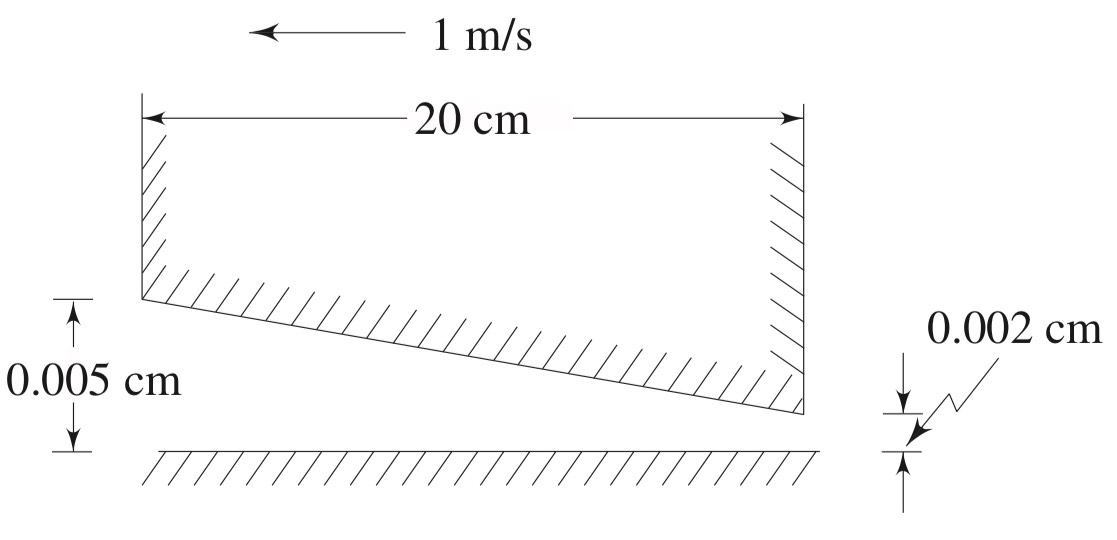
\includegraphics[scale=0.83]{Problem5.jpg}
    \caption{Illustration of Problem 5}
    \label{fig:figprob5}
\end{figure}

Find out the
\begin{enumerate}[noitemsep, nosep]
    \item load carrying capacity of the bearing
    \item drag
    \item power lost in the bearing 
\end{enumerate}

\hfill

\textbf{\underline{Answer}}

Assumptions:
\begin{enumerate}[noitemsep, nosep]
    \item Incompressible fluid
    \item Steady state flow
\end{enumerate}

\hfill

Governing Equation:
\begin{enumerate}[noitemsep, nosep]
    \item Navier-Stokes Equation
    \begin{equation}
        \rho \frac{d \mathbf{v}}{dt} = -\mathbf{\nabla}p + \mu \nabla^2 \mathbf{v} + \rho \mathbf{g}
    \end{equation}

    and in Cartesian coordinate system, in $x-$direction
    \begin{equation}
        \rho \left( \frac{\partial v_x}{\partial t} + v_x \frac{\partial v_x}{\partial x} + v_y \frac{\partial v_x}{\partial y} + v_z \frac{\partial v_x}{\partial z} \right) = -\frac{\partial p}{\partial x} + \mu \left(\frac{\partial^2 v_x}{\partial x^2} + \frac{\partial^2 v_x}{\partial y^2} + \frac{\partial^2 v_x}{\partial z^2} \right) + \rho g_x
    \end{equation}
\end{enumerate}

\hfill

Analysis:

Using (11), as there is viscosity, we get that
\begin{align*}
    \rho \left( 0 + v_x \frac{\partial v_x}{\partial x} + 0 + 0 \right) = -\frac{\partial p}{\partial x} + \mu \left(\frac{\partial^2 v_x}{\partial x^2} + \frac{\partial^2 v_x}{\partial y^2} + 0 \right) + 0
\end{align*}
Here, we see that there exists $v_x$ gradient in $x-$direction. However, let's assume that value is small and neglect it. Then, we get that
\begin{align*}
    \frac{\partial p}{\partial x} &= \mu \frac{\partial^2 v_x}{\partial y^2} \\
    v_x (y) &= \frac{1}{2\mu}\frac{\partial p}{\partial x} y^2 + c_1 y + c_2
\end{align*}
Using BCs of:
\begin{enumerate}[noitemsep, nosep]
    \item $v_x = 0$ at $y = 0$
    \item $v_x = U$ at $y = h$
\end{enumerate}
we get that
\begin{align*}
    0 &= 0 + 0 + c_2 \\
    c_2 &= 0 \\
    U &= \frac{1}{2\mu}\frac{\partial p}{\partial x} h^2 + c_1 h \\
    c_1 &= \frac{U}{h} - \frac{1}{2\mu}\frac{\partial p}{\partial x} h
\end{align*}
thus
\begin{align*}
    v_x (y) &= \frac{1}{2\mu}\frac{\partial p}{\partial x} y^2 + \left(\frac{U}{h} - \frac{1}{2\mu}\frac{\partial p}{\partial x} h\right) y \\
    v_x (y) &= U\frac{y}{h} + \frac{1}{2\mu}\frac{\partial p}{\partial x}\left(y^2 - yh\right)
\end{align*}



\end{document}